\documentclass[11pt,a4paper]{article}
\usepackage[margin=2.2cm]{geometry}
\usepackage[T1]{fontenc}
\usepackage{lmodern}
\usepackage{microtype}
\usepackage{graphicx}
\usepackage{booktabs}
\usepackage{tabularx}
\usepackage{multirow}
\usepackage{xcolor}
\usepackage{caption}
\usepackage{enumitem}
\usepackage{amsmath}
\usepackage{pdflscape}
\usepackage[colorlinks=true,linkcolor=blue!50!black,urlcolor=blue!50!black,citecolor=blue!50!black]{hyperref}
\setlist{itemsep=2pt,topsep=3pt}
\captionsetup{font=small,labelfont=bf}
\newcommand{\eps}{\varepsilon}
\newcommand{\good}[1]{\textbf{#1}}
\definecolor{ours}{RGB}{214,96,0}

\title{\textbf{Follow the Money Without Moving the Data}\\[2pt]
\large Privacy-limited questions between banks, planned by an LLM agent, for anti-money-laundering}
\author{Team \emph{Cache me if you can}: Abhishek, Bhavya, Shreyas Deb, Akshat Srivastava\\
LMA Group Project 2026\\[3pt]
\small Code: \url{https://github.com/BhavyaV05/Transaction-Thieves} (see \texttt{README.md} for reproduction)}
\date{11 November 2026}

\begin{document}
\maketitle

\begin{abstract}
\noindent Launderers move money through several banks because each bank sees only its own customers, and banks may not pool their data. This project built and tested a system in which a bank asks partner banks small, private questions about a suspicious transaction. No transaction record leaves the partner bank. An LLM agent (Gemma~4 12B) picks or writes each question. The partner answers with one number, with noise added for privacy. Every question must first prove useful on past alerts, and a fitted formula, not the LLM, makes the final call. The data are IBM's synthetic AMLworld transactions, split into 30 banks. Four detection models and two federated baselines were reproduced, thirteen published LLM agents were run under the same rules, and ten hypotheses were fixed in advance before the test data were used once. The main result is negative. On 771 test alerts the system closes $-0.007$ [$-0.038$, $0.026$] of the gap between a bank working alone and a model that sees every bank. Even the raw records of three partner banks close only 0.04. The system does beat the strongest published agent, BED-LLM ($p=0.004$ after correction for multiple tests). The diagnostics show why: partner answers add little to what the home bank already knows, and the evidence weights learned on past alerts do not hold on the hard alerts the agent handles.
\end{abstract}

%=====================================================================
\section{Introduction}

Money laundering is a network crime. A scheme moves money through many accounts, often at different banks, so no single bank sees the whole pattern. Altman et al.\ showed that a detection model trained on one bank's part of the transaction graph does far worse than the same model trained on the whole graph~\cite{altman2023}. Banks cannot pool their data. US law (section~314(b) of the PATRIOT Act~\cite{cfr314b}) and Singapore's COSMIC platform~\cite{cosmic} let banks share information about suspected laundering, but these requests are slow, manual and often send raw records.

This project tests a middle ground. When a bank's own model is unsure about an alert, an agent at that bank (the \emph{home bank}) may send a partner bank a fixed-form question, such as ``did the receiving account pass on at least 80\% of what it received within 24 hours?''. The partner runs the question on its own ledger and returns one value (yes/no, a count, or the size of an overlap between two account sets). Noise is added under differential privacy~\cite{dwork2014}, so a single answer reveals little about any one transaction. The home bank combines the answers with its own score and decides.

Three design rules set the system apart:
\begin{enumerate}
\item \textbf{Test a question before trusting it.} Every question, including new ones the LLM writes, must first show on past alerts that its answer separates laundering from clean cases. A question that fails cannot affect the decision.
\item \textbf{A formula decides, not the LLM.} The LLM plans what to ask. A fitted formula turns the answers into the final probability, using numbers only. Sharma found that an LLM investigator made worse calls than the model it was helping, because it trusted its own reasoning~\cite{sharma2026}.
\item \textbf{The same rules for every agent.} The planner and every published agent it is compared with use the same compliance check, privacy budget, simulated banks, LLM and call limits. Only the strategy differs.
\end{enumerate}

\paragraph{Why the problem is hard.} Laundering is rare (about one transaction in a thousand), so labels are few and results are noisy. Each answer costs privacy budget and carries noise, so only one or two questions fit per alert. Partner banks reply late or not at all. Text from another bank may hide instructions aimed at the LLM, so free text must never reach the decision.

\noindent The research questions were: (RQ1) how much of the gap between one bank and a model that sees all banks can private questions close; (RQ2) does an LLM choose questions better than simple rules; (RQ3) does testing questions first matter; and (RQ6) how does the system compare with published agents. The ten hypotheses (H1--H10) and their tests were fixed and locked with a hash before the test data were opened.

\paragraph{Contributions.} (1) A complete test bed for private questions between banks, from question language to LLM planner. (2) Reproductions of the main AML baselines on a split that respects time, showing that the official GNN loaders leak future data. (3) Thirteen published LLM agents run under the same LLM, rules and budget. (4) One test run under a locked plan, with its negative result reported in full and explained.

%=====================================================================
\section{Literature Review}

\paragraph{AML data and detection models.} AMLworld~\cite{altman2023} is IBM's synthetic multi-bank transaction dataset, with laundering labels and pattern types. Its reference model is gradient-boosted trees on features from the Graph Feature Preprocessor (GFP)~\cite{blanusa2024}. Graph neural networks report higher scores: Multi-GNN~\cite{egressy2024}, MEGA-GNN~\cite{bilgi2025} and FraudGT~\cite{lin2024}. Each sees either one bank or the whole graph; none queries other banks while their data stay put.

\paragraph{Learning across banks in private.} Project Aurora~\cite{aurora} and Tian et al.~\cite{tian2025} study collaboration between institutions. Ceydeli et al.~\cite{ceydeli2026} exchange GNN layer outputs between banks. Federated averaging with private training (DP-FedAvg) is the standard private baseline. In all of these, banks train one model together; none asks a question per alert. The overlap questions follow the private set-intersection method of Purcell et al.~\cite{purcell2023}, with its noisy output simulated.

\paragraph{LLM agents for fraud and AML.} Sharma~\cite{sharma2026} pairs graph features with an LLM case investigator. Torres et al.~\cite{torres2026} sort AML alerts using subgraph evidence. FinFRE-RAG~\cite{tan2026} retrieves similar fraud cases, and Co-Investigator drafts suspicious-activity reports. All of them work inside one bank and use evidence without testing it first.

\paragraph{General agents and choosing what to ask.} ReAct~\cite{yao2023}, Reflexion~\cite{shinn2023}, ReWOO~\cite{xu2023}, LATS~\cite{zhou2024} and LLMCompiler~\cite{kim2024} are general tool-using loops. DSPy~\cite{khattab2024} tunes a ReAct agent's prompts. BED-LLM~\cite{choudhury2025} and Uncertainty of Thoughts~\cite{hu2024uot} pick the next question by expected information gain, the idea closest to this project, but neither was tested where each question costs privacy and answers are noisy and late.

\paragraph{Keeping an LLM's ideas only if they pass a test.} CAAFE~\cite{hollmann2023} keeps LLM-proposed features only if they improve validation scores, and POPPER~\cite{huang2025} tests hypotheses with e-values. This project applies the same idea to LLM-written questions. The strategy library follows ReasoningBank~\cite{ouyang2026}, and the evidence retriever builds on SubgraphRAG~\cite{li2025} and G-Retriever~\cite{he2024}.

%=====================================================================
\section{Dataset Created / Used}

\paragraph{Source data.} IBM AMLworld~\cite{altman2023}, in its high-laundering versions \textbf{HI-Small} (about 5 million transactions, 0.5 million accounts) and \textbf{HI-Medium} (about 32 million transactions, 2 million accounts). About one transaction in a thousand is laundering. HI-Medium is the main dataset; HI-Small served for development and for baselines that do not scale.

\paragraph{What was built on top.} The raw data are one global ledger, so the multi-bank setting was created for this project:
\begin{itemize}
\item \textbf{Bank views.} Each of the 30 largest banks gets a private view with only the transactions that touch its customers. Each one can act as home bank or as a simulated partner with its own ledger, reply delays, refusals and an optional free-text note, which serves the prompt-injection tests.
\item \textbf{Split by time.} Days 1--9 are training, 10--12 validation and 13--16 test. Every tool takes the alert time and cannot see later data. Code locks the test split, and only the final-run script opened it.
\item \textbf{Alerts.} The home bank's GFP model scores every transaction. A filter keeps only the transactions the model is unsure about. On HI-Medium test this gives \textbf{4,478 alerts}: 3,873 in the main period (975 laundering) and 605 in the sparse final days, reported separately.
\item \textbf{Askable alerts.} A question needs a partner bank that holds the other account. Of the 3,873 main alerts, \textbf{771} are askable (241 laundering). A random subset of 1,000 test alerts, fixed in advance, contains 208 askable ones and serves the more expensive agents.
\item \textbf{Question table and strategy library.} Training-period alerts gave a table of 440 question and privacy-level pairs with their tested evidence weights (23 accepted on HI-Medium), and a library of question strategies indexed by the \emph{shape} of the local graph, never by account.
\end{itemize}

%=====================================================================
\section{Methodology}

\begin{figure}[t]
\centering
\small
\setlength{\fboxsep}{6pt}
\fbox{\parbox{0.93\linewidth}{\centering\footnotesize
\textbf{Home bank}: alert intake (GFP score $p_0$ + filter for unsure cases) $\rightarrow$ evidence retriever (40 time-ordered edges)
$\rightarrow$ \textcolor{ours}{\textbf{LLM planner}} (Gemma 4 12B, LangGraph; strategy library + regulation lookup)\\[3pt]
$\downarrow$ fixed-form question (program, bank, $\eps$, legal basis)\\[3pt]
\textbf{Compliance check + privacy accounting} (allowlist; $\eps\in\{0.25,0.5,1,2\}$; 2 per alert; cap 8 per partner account)\\[3pt]
$\downarrow$\\[3pt]
\textbf{Partner bank} (runs the question on its own ledger up to the alert time; adds noise; delays, refusals; one value back)\\[3pt]
$\downarrow$ noisy answer $\rightarrow$ tested evidence weight\\[3pt]
\textcolor{ours}{\textbf{Fitted decision formula}} (numbers only, no LLM text) $\rightarrow$ probability $\hat p$ $\rightarrow$ stop / ask again / decide
}}
\caption{The path of one alert through the system. No transaction record leaves a partner bank, and the LLM never writes the final probability.}
\label{fig:arch}
\end{figure}

Figure~\ref{fig:arch} shows the pipeline. Its starting point is $p_0$, the probability of laundering that the home bank's own GFP model gives an alert.

\paragraph{Questions and privacy.} A question is a short program in a small question language. It refers to accounts by their role in the alert (``the receiver''), never by account number or date. The partner answers yes/no with a set chance of flipping it, or returns a count with random noise added. Privacy is counted per transaction: at most $\eps=2$ per alert, and at most $\eps=8$ per partner account over the whole test period. A smaller $\eps$ means more noise and more privacy.

\paragraph{Compliance check.} Every question, from the planner or from a published agent, passes the same checks: a known partner, an allowed $\eps$, a valid program, a legal basis from 314(b) or MAS COSMIC, and enough budget left. The LLM sees only random aliases of accounts.

\paragraph{Testing questions first.} For each question and $\eps$ level, the question is replayed on past training alerts with the same noise. This gives its \emph{likelihood ratio}: how much more often each answer occurs for laundering than for clean alerts. A question is \emph{accepted} only if it passes a test that limits false discoveries~\cite{wang2022}, and its ratio is capped at the most that $\eps$ allows. New questions the LLM writes must pass the same test before their answers count.

\paragraph{Decision formula.} The final probability is $\operatorname{logit}\hat p = \operatorname{logit} p_0 + \sum_k w_{f(k)} \log \mathrm{LR}_k$: the home bank's score, moved by the weighted evidence of each answer. There is one weight per question family, fitted on validation and then frozen. With all weights set to 1, the formula moved $p_0$ the wrong way on validation, because the questions partly measure what $p_0$ already knows. Fitted weights fixed this before the test run.

\paragraph{Planner.} The planner is built with LangGraph around Gemma~4 12B. At each step it sees the evidence, $p_0$, the current probability, the remaining budget and a menu of strategies. It then picks a listed question, writes a new one, or stops. Its free text is logged but never enters the decision. A size sweep of seven models, planned in advance (E18), chose the backbone.

\paragraph{Baselines.} Five planners without an LLM run in the same system: random, a fixed expert order, expected information gain, a learned policy, and an enumerator that tries every question. \emph{Raw sharing} gives the home bank the actual records of three partner banks with no noise; it shows the most that sharing could add. The thirteen published agents (Table~\ref{tab:valagents}) each run \emph{as published} (one bank's view) and \emph{ported} (with the question tool and budget). \emph{Adapted} versions run an agent's control loop inside this system, which separates a better loop from better evidence weights.

\paragraph{Measuring success.} The main measure is the Brier score, the mean squared error of the predicted probability (lower is better). From it comes the \emph{gap closed}:
\[
G = \frac{B(\text{one bank}) - B(\text{system})}{B(\text{one bank}) - B(\text{see everything})},
\]
where ``see everything'' is GFP trained on all banks' data. $G=0$ means no gain over the bank alone, and $G=1$ means as good as pooling all data. Intervals are 95\% bootstrap intervals, and p-values are Holm-corrected for multiple tests. All thresholds and the choice of the best published agent were fixed on validation.

%=====================================================================
\section{Experiment Runs}
\label{sec:exp}

Table~\ref{tab:scale} sums up the work. Most of it ran on an RTX 5070 Ti, the rest on a 3070 Ti laptop and the \emph{ada} HPC cluster.

\begin{table}[h]
\centering\small
\begin{tabularx}{\linewidth}{lX}
\toprule
Work item & Scale \\
\midrule
Detection baselines & 4 models (GFP, Multi-GNN, MEGA-GNN, FraudGT), one bank and see everything, on HI-Small and HI-Medium; FraudGT 500 epochs \\
Federated baselines & DP-FedAvg: 2 privacy units $\times$ 6 $\varepsilon$ levels $\times$ 3 seeds; layer-wise exchange: 8 versions $\times$ 3 seeds \\
Backbone sweep (E18) & 7 open LLMs on 160, then 460 validation alerts; 4.6 GPU-hours \\
Fine-tuning & QLoRA Qwen3-8B student $\times$ 3 seeds; Qwen3-4B fast model; DSPy prompt tuning (2.7 GPU-hours) \\
Agents and validation & 13 published agents, 27 agent versions; 33 systems on validation; about 60 GPU-hours \\
Safety & Prompt-injection tests (E15) with 4 attack types \\
Final test run & 25 systems, 12,040 verdicts, 44 GPU-hours, run once after the lock \\
Engineering & 3 machines; about 600 commits and 158 pull requests by four people; 1,243 unit tests \\
\bottomrule
\end{tabularx}
\caption{The scale of the work behind this report.}
\label{tab:scale}
\end{table}

\paragraph{Reproducing the detection baselines.} On the paper's own split, GFP + LightGBM scored F1 62.95 (published 62.86 $\pm$ 0.25), GFP + XGBoost 62.51 (63.23), and Multi-GNN with the official code 67.64 (68.16 $\pm$ 2.65). MEGA-GNN was only partly reproduced (59.7 vs.\ 74.88 after 10 of 80 epochs, for lack of compute). FraudGT ran its full 500 epochs (best validation F1 0.686). All models were then retrained, one bank and see everything, on the time-based split. The official GNN loaders sample future edges, so their see-everything scores are too high. With future edges removed, Multi-GNN's HI-Medium PR-AUC drops from 0.611 to 0.199. GFP therefore serves as the upper limit.

\paragraph{Federated baselines.} DP-FedAvg ran with privacy per bank and per transaction, $\eps$ from 1 to 16 plus a no-noise version, three seeds each. The layer-wise exchange of Ceydeli et al.\ ran in eight versions. On HI-Small validation, the best layer-wise version beat one-bank GFP by a small margin (Brier 0.001116 vs.\ 0.001167). DP-FedAvg with real privacy did not reach one-bank GFP, and the per-transaction version fell to the base rate.

\paragraph{Backbone sweep (E18).} Seven open models were tried as planners on 160 validation alerts, and the best three on 460. Gemma~4 12B won (Brier 0.1741, against 0.1844 for Qwen3.8-27B and 0.1890 for Qwen3-14B). gpt-oss-20b gave invalid outputs, and a ``thinking'' version never answered.

\paragraph{Fine-tuning.} The planner's successful steps trained a smaller QLoRA~\cite{hu2022lora,dettmers2023} student (Qwen3-8B, three seeds), and a Qwen3-4B fast model handled routine decisions. The students learned the output format but planned worse than the 12B model (Brier 0.223--0.226 vs.\ 0.201 on 160 validation alerts). Used as an injection filter, the fast model cut ReAct's prompt-injection success from 5--8\% to 0\%.

\paragraph{The final run.} After the plan was locked, one script ran each system once on the test split: the system at $\eps\in\{1,2,4\}$, four ablations, five planners without an LLM, raw sharing, BED-LLM on all askable alerts, and Co-Investigator plus two adapted agents on the subset. A reduced plan, fixed in advance, was run because of the deadline; the full plan needed about 188 GPU-hours.

%=====================================================================
\section{Evaluations}

\begin{table}[t]
\centering\small
\resizebox{\linewidth}{!}{\begin{tabular}{llrrl}
\toprule
& Hypothesis (test) & Estimate [95\% CI] & $p_\text{Holm}$ & Verdict \\
\midrule
H1 & Gap closed vs.\ one bank & $-0.007$ [$-0.038$, 0.026] & 1.00 & not supported \\
H2 & Benefit relative to raw sharing & $-0.165$ [$-2.88$, 0.75] & 1.00 & not supported \\
H3 & LLM planner beats simple planners & $-0.001$ [$-0.006$, 0.003] & 0.33 & not supported \\
H4 & Testing questions helps (+ false-discovery audit) & $-0.005$ [$-0.010$, $-0.000$] & 0.072 & not supported \\
\textbf{H9} & \textbf{Beats best published agent (BED-LLM)} & \textbf{0.266} [$-0.022$, 0.799] & \textbf{0.004} & \textbf{supported} \\
H7 & Formula vs.\ LLM deciding & $-0.000$ [$-0.004$, 0.004] & 1.00 & not supported \\
\bottomrule
\end{tabular}}
\caption{Hypotheses fixed in advance, on the test split (771 askable alerts; H9's interval is for the difference in gap closed). H5, H6, H8 and H10 were not run in the reduced plan.}
\label{tab:hyp}
\end{table}

\paragraph{What counts as a result.} Only the tests in Table~\ref{tab:hyp} are confirmatory. Everything else, including the ablations and the appendix, is exploratory and never changes a verdict.

\paragraph{Detection models.} On all 3,873 main alerts, one-bank GFP has Brier 0.1585 (PR-AUC 0.602) and see-everything GFP 0.0854 (PR-AUC 0.848). This is the gap to close, and it is large: if reviewers check the top 10\% of alerts, the see-everything model is right on 98\% of them, against 72\% for one bank.

\begin{table}[t]
\centering\small
\begin{tabular}{llrrrr}
\toprule
Group & System & Brier & Gap closed [95\% CI] & Qs/alert & $\eps$ spent \\
\midrule
Reference & One bank only & 0.1668 & 0 & -- & -- \\
& See everything (GFP) & 0.0966 & 1 & -- & -- \\
& Raw records, 3 banks, no noise & 0.1640 & 0.040 [$-0.107$, 0.161] & 1.99 & 0 \\
\midrule
No LLM & Random & 0.1698 & $-0.042$ [$-0.102$, 0.005] & 5.12 & 1.83 \\
& Fixed expert order & 0.1694 & $-0.036$ [$-0.072$, $-0.012$] & 2.33 & 1.89 \\
& Expected info.\ gain & 0.1823 & $-0.220$ [$-0.392$, $-0.114$] & 8.80 & 1.44 \\
& Learned policy & 0.1814 & $-0.207$ [$-0.369$, $-0.103$] & 7.99 & 1.45 \\
& Enumerator & 0.1708 & $-0.057$ [$-0.178$, 0.055] & 1.78 & 0.69 \\
\midrule
Published & BED-LLM (frozen pick) & 0.1956 & $-0.410$ [$-0.831$, $-0.176$] & 2.76 & 0.61 \\
\midrule
\textcolor{ours}{\textbf{Proposed}} & \textbf{Write questions, $\eps=2$} & \textbf{0.1673} & $\mathbf{-0.007}$ [$-0.038$, 0.026] & 1.55 & 1.46 \\
& Budget $\eps=1$ & 0.1666 & 0.004 [$-0.025$, 0.031] & -- & 0.74 \\
& Budget $\eps=4$ & 0.1679 & $-0.015$ [$-0.057$, 0.030] & -- & 2.67 \\
\bottomrule
\end{tabular}
\caption{Test results on the 771 askable alerts (lower Brier is better). The appendix (Tables~\ref{tab:big}--\ref{tab:valagents}) lists every system on every metric, on test and validation.}
\label{tab:main}
\end{table}

\paragraph{Main result (H1, H2).} Table~\ref{tab:main} shows the headline. The system's Brier (0.1673) is the same, within noise, as the bank working alone (0.1668): it closes none of the gap. Raw, noise-free records from three partner banks close only 4\% of it, and that interval also covers zero. So privacy noise is not the main limit: what a partner bank knows about one account adds little to what GFP already computes from the home bank's graph. The flat privacy curve ($\eps=1$, 2 and 4 lie within 0.0013 Brier) fits that reading.

\paragraph{Planners (H3).} The LLM planner beats every simple planner except the enumerator. Expected information gain and the learned policy ask many questions and do much worse. H3 required beating the enumerator too, so it is not supported.

\begin{table}[t]
\centering\small
\resizebox{\linewidth}{!}{\begin{tabular}{lrrrrr}
\toprule
Agent (subset, 208 askable) & Brier & Gap closed [95\% CI] & LLM calls & GPU-s/alert & No verdict \\
\midrule
\textbf{This system, write questions} & \textbf{0.1576} & \textbf{0.005} [$-0.044$, 0.058] & 2.4 & 28.4 & 0 \\
DSPy ReAct (adapted) & 0.1623 & $-0.051$ [$-0.149$, 0.033] & 1.4 & 7.4 & 0 \\
ReWOO (adapted) & 0.1638 & $-0.068$ [$-0.145$, $-0.007$] & 0.9 & 4.1 & 0 \\
BED-LLM & 0.1805 & $-0.262$ [$-0.797$, 0.026] & 6.9 & 32.9 & 0 \\
Co-Investigator & 0.2334 & $-0.878$ [$-1.709$, $-0.471$] & 7.6 & 38.7 & 0.71 \\
\bottomrule
\end{tabular}}
\caption{Published agents against this system on the same 208 askable subset alerts, with the same LLM, rules and budget.}
\label{tab:ext}
\end{table}

\paragraph{Published agents (H9).} Here the system wins (Table~\ref{tab:ext}, Figure~\ref{fig:figs}). On all 771 askable alerts it beats BED-LLM, the strongest published agent on validation, by 0.27 in gap closed (Holm $p=0.004$). BED-LLM and Co-Investigator make the final call themselves and drift away from $p_0$; Co-Investigator gives no usable verdict on 71\% of alerts. The adapted agents, which use this system's formula, come much closer, so most of the advantage comes from the tested weights and the formula, not from a smarter loop. Scored on their questions alone, all systems fall far below zero, this one included.

\begin{figure}[t]
\centering
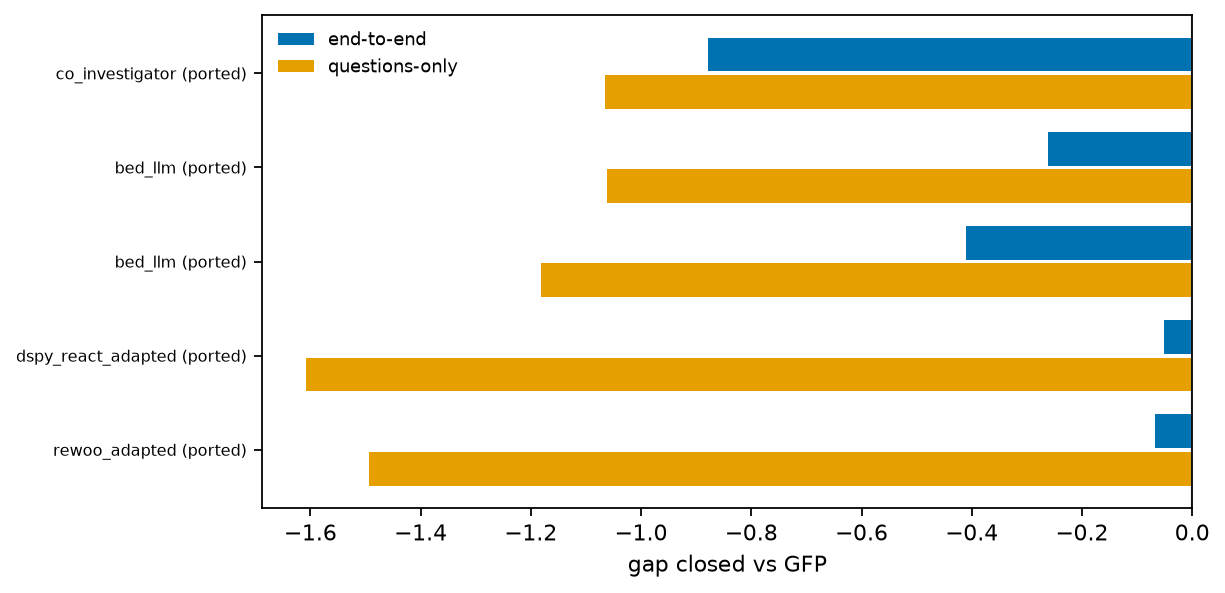
\includegraphics[width=0.53\linewidth]{figures/external_gap.png}\hfill
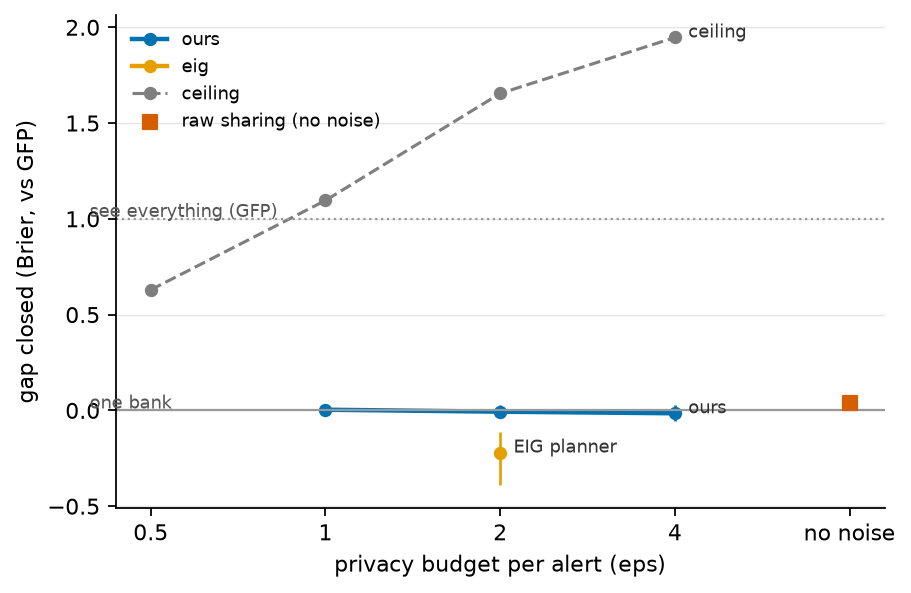
\includegraphics[width=0.42\linewidth]{figures/privacy_curve.png}
\caption{Left: gap closed by each published agent and by this system (end to end, and on questions only). Right: the system's privacy curve on the 771 test alerts is flat.}
\label{fig:figs}
\end{figure}

\paragraph{Cost and safety.} The planner uses 2.4 LLM calls, about 12,900 tokens and 29 GPU-seconds per alert, and spends $\eps\approx1.46$ of its budget of 2. BED-LLM makes three times the calls for a worse result. On \emph{all} 3,873 alerts (alerts that cannot be asked about keep $p_0$), the system differs from one bank by $+0.0001$ [$-0.0003$, 0.0005] Brier, so it does no harm. BED-LLM is worse by $+0.0057$ [0.003, 0.008] and Co-Investigator by $+0.0157$.

%=====================================================================
\section{Ablations}

Each part was switched off in turn, on the same 208 askable subset alerts (Table~\ref{tab:abl}).

\begin{table}[h]
\centering\small
\resizebox{\linewidth}{!}{\begin{tabular}{lrrrl}
\toprule
Ablation & Brier & $\Delta$ vs.\ full system [95\% CI] & Qs/alert & Reading \\
\midrule
Full system (write questions) & 0.1576 & -- & 1.53 & \\
LLM may only pick from a fixed list & 0.1656 & +0.0080 [0.0031, 0.0131] & 1.18 & \good{writing questions helps} \\
No question testing (LLM's own belief) & 0.1626 & +0.0049 [0.0003, 0.0099] & 2.71 & \good{testing helps} \\
Act only, no stated hypothesis & 0.1592 & +0.0016 [$-0.0026$, 0.0059] & 1.46 & small, not significant \\
LLM decides when to stop or escalate & 0.1577 & +0.0001 [$-0.0035$, 0.0038] & 1.52 & no difference \\
\bottomrule
\end{tabular}}
\caption{Ablations (a positive $\Delta$ means the ablation does worse than the full system).}
\label{tab:abl}
\end{table}

Two parts earn their place. Letting the LLM \emph{write} new questions, instead of picking from a fixed list, lowers Brier by 0.008, with an interval that excludes zero. Without \emph{question testing}, the system asks almost twice as many questions, uses twice the LLM calls and GPU time, and does worse by 0.005. In the H4 test on all 771 alerts this effect was $-0.005$ [$-0.010$, $-0.000$] (Holm $p=0.072$), and H4 also needed a check on false discoveries among accepted questions, which failed (0.714). Stating a hypothesis before acting, and letting the LLM decide when to stop (H7), made no measurable difference. The privacy budget variants ($\eps=1$, 2, 4) are in Table~\ref{tab:main}.

%=====================================================================
\section{Limitations}\label{sec:lim}

\begin{itemize}
\item \textbf{Synthetic data, simulated banks.} AMLworld is generated, and the partner banks, delays and set overlaps are simulated. Real requests between banks, and real laundering, are messier.
\item \textbf{Privacy unit.} The guarantee is per transaction, not per customer; the cap of $\eps=8$ per account is a partial fix.
\item \textbf{Reduced final run.} For lack of time, a subset of systems fixed in advance was run. H5, H6, H8 and H10, the evidence-view versions, the fine-tuned students and $\eps=0.5$ and $\infty$ were not run on test, and only one published agent ran on all askable alerts.
\item \textbf{Recorded deviations.} Two reruns did not exactly match their validation scores and were kept with a recorded deviation: see-everything GFP on HI-Medium, and layer-wise exchange on HI-Small (dropped on HI-Medium). FraudGT was scored once before the lock, the CPU planners were rerun once, and a few test-path bugs were fixed during the final run without changing any locked setting. The plan had no TA countersignature.
\end{itemize}

%=====================================================================
\section{Conclusions: lessons from a system that did not work}

The idea did not work. Under a locked plan, an LLM agent asking partner banks private questions did not improve on the bank's own GFP model (H1), and only one primary hypothesis held (H9, against other LLM agents).

\paragraph{1. Partner banks had little to add.} Even raw, noise-free records from three partner banks closed only 4\% of the gap, with an interval covering zero. The see-everything model gains from patterns that span many hops across the whole network, while one partner can describe only one account one hop away. GFP's own features (money in and out, counts, local cycles) already capture most of that hop, so the questions re-measured much of what $p_0$ knew. The main lesson: measure how much a partner's view adds beyond the home bank's features before building the question machinery, and redesign if the answer is small.

\paragraph{2. Evidence weights from past alerts did not carry over.} On validation, the summed evidence did not predict the labels (fitted slope $-0.03$, where 1 means the weights hold), and most question families pointed the right way only about half the time. The weights came from past training alerts, but the alerts that reach the agent are the hard, ambiguous ones the filter lets through, and the data change over time. Fitting the weights only shrank the damage to zero.

\paragraph{3. Too few alerts could be asked about.} With only 771 of 3,873 alerts askable, even a perfect system could move at most a fifth of the headline. With 241 laundering cases, the smallest detectable effect was larger than any effect seen.

\paragraph{4. Privacy caps what one answer can say.} With $\eps\le2$, a yes/no answer can shift the odds by at most $e^{\eps}$; the strongest accepted answer shifted them by a factor of 3.8. Privacy was not the limit here, but it would be if the answers were informative.

\paragraph{5. LLMs judge probabilities poorly but can plan.} Every published agent that writes its own probability ranked alerts worse than $p_0$ on validation (AUC 0.29--0.72 against 0.76). On test, BED-LLM and Co-Investigator did worse than the bank alone. The same loops run inside this system (the adapted versions) matched $p_0$. Question testing and the formula kept the system from hurting the base model, which is why H9 holds. Writing and testing new questions both helped, so the LLM's planning had value, with little signal to work on. The QLoRA student, trained on 252 examples, learned the format but not the policy.

\paragraph{6. Engineering.} Locking the plan and the test data kept the evaluation honest when the results disappointed. The time between the first full end-to-end number and the lock was too short: the key diagnostic (point 2) appeared late in validation. Reproducing every baseline first cost GPU days but exposed the future-edge leak in the official GNN loaders, which inflates see-everything scores.

\paragraph{Next steps.} Measure partner information first. Ask about what the home bank \emph{cannot} compute, such as cycles that cross several banks. Estimate evidence weights on the same hard alerts the agent sees, and add more partner banks to raise coverage.

%=====================================================================
\section*{Reproducibility}\sloppy
\begin{itemize}
\item \textbf{Code and data:} \url{https://github.com/BhavyaV05/Transaction-Thieves}; \texttt{README.md} lists every command. AMLworld is public on Kaggle.
\item \textbf{Locked plan:} \texttt{prereg/}, with its hash in \texttt{prereg/FREEZE.json}; only \texttt{scripts/run\_final.py} reads the test split. Trained weights are not released, and FraudGT's patch stays outside the repository because its code has no licence.
\end{itemize}

\small
\begin{thebibliography}{99}\setlength{\itemsep}{1pt}
\bibitem{altman2023} E.~Altman et al. Realistic synthetic financial transactions for anti-money laundering models. NeurIPS Datasets and Benchmarks, 2023.
\bibitem{blanusa2024} J.~Blanu\v{s}a et al. Graph Feature Preprocessor: real-time subgraph-based feature extraction for financial crime detection. arXiv:2402.08593, 2024.
\bibitem{egressy2024} B.~Egressy et al. Provably powerful graph neural networks for directed multigraphs (Multi-GNN). AAAI, 2024.
\bibitem{bilgi2025} H.~\c{C}.~Bilgi et al. Multigraph message passing with bi-directional multi-edge aggregations (MEGA-GNN). arXiv:2412.00241, 2024.
\bibitem{lin2024} J.~Lin et al. FraudGT: a simple, effective, and efficient graph transformer for financial fraud detection. ICAIF, 2024.
\bibitem{sharma2026} R.~Sharma. Toward auditable fraud detection: combining graph features, model explanations, and agentic case investigation. arXiv:2607.19266, 2026.
\bibitem{torres2026} D.~Torres, W.~Cheng, K.~Hu. Explainable AML triage with LLMs: evidence retrieval and counterfactual checks. arXiv:2604.19755, 2026.
\bibitem{tan2026} X.~Tan, Y.~Ma, X.~Zhang. Understanding structured financial data with LLMs: a case study on fraud detection (FinFRE-RAG). ACL, 2026.
\bibitem{aurora} Bank for International Settlements. Project Aurora: the power of data, technology and collaboration to combat money laundering across institutions and borders. 2023.
\bibitem{tian2025} Z.~Tian et al. Towards collaborative anti-money laundering among financial institutions. WWW, 2025.
\bibitem{ceydeli2026} Ceydeli, Wang, Atasu. Federated layer-wise exchange for cross-client money laundering pattern detection. arXiv:2605.06433, 2026.
\bibitem{purcell2023} C.~Purcell et al. Split, count, and share: a differentially private set intersection cardinality estimation protocol. UAI, 2023.
\bibitem{dwork2014} C.~Dwork, A.~Roth. The algorithmic foundations of differential privacy. Foundations and Trends in TCS, 2014.
\bibitem{wang2022} R.~Wang, A.~Ramdas. False discovery rate control with e-values. JRSS-B, 2022.
\bibitem{huang2025} K.~Huang et al. Automated hypothesis validation with agentic sequential falsifications (POPPER). ICML, 2025.
\bibitem{hollmann2023} N.~Hollmann, S.~M\"uller, F.~Hutter. Large language models for automated data science: CAAFE. NeurIPS, 2023.
\bibitem{choudhury2025} D.~Choudhury et al. BED-LLM: intelligent information gathering with LLMs and Bayesian experimental design. arXiv:2508.21184, 2025.
\bibitem{hu2024uot} Z.~Hu et al. Uncertainty of Thoughts: uncertainty-aware planning enhances information seeking in LLMs. NeurIPS, 2024.
\bibitem{yao2023} S.~Yao et al. ReAct: synergizing reasoning and acting in language models. ICLR, 2023.
\bibitem{shinn2023} N.~Shinn et al. Reflexion: language agents with verbal reinforcement learning. NeurIPS, 2023.
\bibitem{xu2023} B.~Xu et al. ReWOO: decoupling reasoning from observations for efficient augmented language models. arXiv:2305.18323, 2023.
\bibitem{zhou2024} A.~Zhou et al. Language Agent Tree Search (LATS). ICML, 2024.
\bibitem{kim2024} S.~Kim et al. An LLM compiler for parallel function calling. ICML, 2024.
\bibitem{khattab2024} O.~Khattab et al. DSPy: compiling declarative language model calls into self-improving pipelines. ICLR, 2024.
\bibitem{ouyang2026} S.~Ouyang et al. ReasoningBank: scaling agent self-evolving with reasoning memory. ICLR, 2026.
\bibitem{li2025} M.~Li, S.~Miao, P.~Li. Simple is effective: the roles of graphs and LLMs in KG-based RAG (SubgraphRAG). ICLR, 2025.
\bibitem{he2024} X.~He et al. G-Retriever: retrieval-augmented generation for textual graph understanding. NeurIPS, 2024.
\bibitem{hu2022lora} E.~J.~Hu et al. LoRA: low-rank adaptation of large language models. ICLR, 2022.
\bibitem{dettmers2023} T.~Dettmers et al. QLoRA: efficient finetuning of quantized LLMs. NeurIPS, 2023.
\bibitem{cfr314b} 31 CFR 1010.540. Voluntary information sharing among financial institutions (314(b)). U.S. Code of Federal Regulations.
\bibitem{cosmic} Monetary Authority of Singapore. Guidelines on COSMIC (Collaborative Sharing of ML/TF Information and Cases). 2024.
\end{thebibliography}
\normalsize
\clearpage
\appendix
\section{Full comparison tables}

\begin{landscape}
\begin{table}
\centering
\caption{\textbf{Every tested model against this system, on every metric} (test split, HI-Medium, frozen final run g5, $\varepsilon=2$ per alert). \textcolor{ours}{\textbf{This system}} is the frozen, pre-registered one; its variants and ablations are in Table~\ref{tab:bigabl}. \textbf{Bold} = best value in each quality column among all systems except the see-everything upper limit ($^\ast$), which needs every bank's data; ties of more than three systems are not marked. $\Delta B$ = Brier minus one bank on the same alerts (negative is better). Gap closed is against GFP see-everything; ``QO'' scores only the system's questions through this system's formula. AUC = ROC-AUC. ECE uses 10 equal-mass bins. P@10\%, R@10\% = precision and recall when the top 10\% of alerts by score are reviewed. No-v. = share of alerts with no usable verdict (scored as $p_0$). Costs are per alert; tokens are input plus output. Non-LLM planners and raw sharing use no LLM. Confidence intervals for the main rows are in Tables~\ref{tab:main} and~\ref{tab:ext}.}
\label{tab:big}
\setlength{\tabcolsep}{3.2pt}
\scriptsize
\resizebox{\linewidth}{!}{\begin{tabular}{llrrrrrrrrrrrrrrr}
\toprule
 & & \multicolumn{4}{c}{Probability quality} & \multicolumn{3}{c}{Ranking and calibration} & \multicolumn{2}{c}{Review at 10\%} & & \multicolumn{5}{c}{Cost per alert} \\
\cmidrule(lr){3-6}\cmidrule(lr){7-9}\cmidrule(lr){10-11}\cmidrule(lr){13-17}
Group & System & Brier & $\Delta B$ & Gap & Gap QO & AUC & PR-AUC & ECE & P@10\% & R@10\% & No-v. & Qs & $\varepsilon$ & LLM calls & Tokens & GPU-s \\
\midrule
\multicolumn{17}{l}{\textit{All 771 askable test alerts (241 laundering)}}\\
Reference & One bank only (GFP $p_0$) & 0.1668 & 0.0000 & 0.000 & -- & 0.809 & 0.660 & \textbf{0.098} & 0.83 & 0.27 & -- & -- & -- & -- & -- & -- \\
 & See everything (GFP, upper limit)$^\ast$ & 0.0966 & $-$0.0702 & 1.000 & -- & 0.915 & 0.876 & 0.055 & 1.00 & 0.32 & -- & -- & -- & -- & -- & -- \\
 & Raw records, 3 banks, no privacy & \textbf{0.1640} & \textbf{$-$0.0028} & \textbf{0.040} & -- & \textbf{0.846} & \textbf{0.731} & 0.140 & 0.83 & 0.27 & 0.00 & 1.99 & 0.00 & -- & -- & -- \\
\addlinespace[3pt]
Non-LLM planners & Random & 0.1698 & 0.0029 & $-$0.042 & $-$1.27 & 0.810 & 0.665 & 0.103 & 0.81 & 0.26 & 0.00 & 5.12 & 1.83 & -- & -- & -- \\
 & Fixed expert order & 0.1694 & 0.0025 & $-$0.037 & $-$1.24 & 0.807 & 0.655 & 0.100 & 0.83 & 0.27 & 0.00 & 2.33 & 1.89 & -- & -- & -- \\
 & Expected information gain & 0.1823 & 0.0154 & $-$0.220 & $-$1.59 & 0.795 & 0.649 & 0.134 & 0.81 & 0.26 & 0.00 & 8.80 & 1.44 & -- & -- & -- \\
 & Learned policy & 0.1814 & 0.0145 & $-$0.208 & $-$1.57 & 0.797 & 0.651 & 0.133 & 0.81 & 0.26 & 0.00 & 7.99 & 1.45 & -- & -- & -- \\
 & Enumerator (every question) & 0.1708 & 0.0040 & $-$0.057 & $-$1.19 & 0.814 & 0.670 & 0.124 & 0.82 & 0.26 & 0.00 & 1.78 & 0.69 & -- & -- & -- \\
\addlinespace[3pt]
External LLM agents & BED-LLM & 0.1956 & 0.0288 & $-$0.410 & \textbf{$-$1.18} & 0.735 & 0.553 & 0.103 & 0.60 & 0.19 & 0.00 & 2.76 & 0.61 & 6.9 & 21.6k & 32.6 \\
\addlinespace[3pt]
\textcolor{ours}{\textbf{This system}} & \textbf{LLM planner, compose, $\varepsilon=2$} & 0.1673 & 0.0005 & $-$0.007 & $-$1.38 & 0.816 & 0.663 & 0.102 & 0.83 & 0.27 & 0.00 & 1.55 & 1.46 & 2.4 & 12.9k & 29.0 \\
\midrule
\multicolumn{17}{l}{\textit{Pre-registered subset: 208 askable test alerts (60 laundering)}}\\
Reference & One bank only (GFP $p_0$) & 0.1580 & 0.0000 & 0.000 & -- & 0.825 & 0.688 & \textbf{0.123} & 0.86 & 0.30 & -- & -- & -- & -- & -- & -- \\
 & See everything (GFP, upper limit)$^\ast$ & 0.0722 & $-$0.0858 & 1.000 & -- & 0.938 & 0.910 & 0.042 & 1.00 & 0.35 & -- & -- & -- & -- & -- & -- \\
 & Raw records, 3 banks, no privacy & \textbf{0.1537} & \textbf{$-$0.0044} & \textbf{0.051} & -- & \textbf{0.872} & \textbf{0.774} & 0.162 & 0.86 & 0.30 & 0.00 & 1.89 & 0.00 & -- & -- & -- \\
\addlinespace[3pt]
Non-LLM planners & Random & 0.1591 & 0.0011 & $-$0.013 & -- & 0.851 & 0.724 & 0.132 & 0.86 & 0.30 & 0.00 & 5.31 & 1.85 & -- & -- & -- \\
 & Fixed expert order & 0.1590 & 0.0010 & $-$0.011 & -- & 0.829 & 0.690 & 0.127 & 0.86 & 0.30 & 0.00 & 2.57 & 1.88 & -- & -- & -- \\
 & Expected information gain & 0.1773 & 0.0193 & $-$0.225 & -- & 0.815 & 0.677 & 0.157 & 0.86 & 0.30 & 0.00 & 8.88 & 1.35 & -- & -- & -- \\
 & Learned policy & 0.1718 & 0.0138 & $-$0.160 & -- & 0.832 & 0.696 & 0.156 & 0.86 & 0.30 & 0.00 & 8.77 & 1.36 & -- & -- & -- \\
 & Enumerator (every question) & 0.1569 & $-$0.0011 & 0.013 & -- & 0.844 & 0.713 & 0.145 & 0.86 & 0.30 & 0.00 & 1.66 & 0.67 & -- & -- & -- \\
\addlinespace[3pt]
External LLM agents & BED-LLM & 0.1805 & 0.0225 & $-$0.262 & \textbf{$-$1.06} & 0.774 & 0.608 & 0.136 & 0.71 & 0.25 & 0.00 & 2.79 & 0.67 & 6.9 & 21.5k & 32.9 \\
 & Co-Investigator & 0.2334 & 0.0754 & $-$0.879 & \textbf{$-$1.06} & 0.756 & 0.555 & 0.219 & 0.71 & 0.25 & 0.71 & 2.27 & 0.97 & 7.6 & 16.9k & 38.7 \\
 & DSPy ReAct (adapted) & 0.1623 & 0.0043 & $-$0.051 & $-$1.61 & 0.832 & 0.700 & 0.145 & 0.86 & 0.30 & 0.00 & 1.30 & 1.63 & 1.4 & 3.0k & 7.4 \\
 & ReWOO (adapted) & 0.1638 & 0.0058 & $-$0.068 & $-$1.49 & 0.834 & 0.692 & 0.141 & 0.86 & 0.30 & 0.00 & 0.89 & 0.85 & 0.9 & 1.8k & 4.1 \\
\addlinespace[3pt]
\textcolor{ours}{\textbf{This system}} & \textbf{LLM planner, compose, $\varepsilon=2$} & 0.1576 & $-$0.0004 & 0.005 & -- & 0.838 & 0.697 & 0.132 & 0.86 & 0.30 & 0.00 & 1.53 & 1.47 & 2.4 & 12.9k & 28.4 \\
\bottomrule
\end{tabular}}
\end{table}
\end{landscape}

\begin{landscape}
\begin{table}
\centering
\caption{\textbf{This system: privacy budget variants and ablations}, same metrics as Table~\ref{tab:big}. The budget rows use all 771 askable test alerts; the ablations use the 208 askable subset alerts (each ablation switches off one component of the full system). \textbf{Bold} = best in each quality column within each block. Intervals for the ablation differences are in Table~\ref{tab:abl}. $\Delta B$ = Brier minus one bank on the same alerts (negative is better). Gap closed is against GFP see-everything; ``QO'' scores only the system's questions through this system's formula. AUC = ROC-AUC. ECE uses 10 equal-mass bins. P@10\%, R@10\% = precision and recall when the top 10\% of alerts by score are reviewed. No-v. = share of alerts with no usable verdict (scored as $p_0$). Costs are per alert; tokens are input plus output.}
\label{tab:bigabl}
\setlength{\tabcolsep}{3.2pt}
\scriptsize
\resizebox{\linewidth}{!}{\begin{tabular}{llrrrrrrrrrrrrrrr}
\toprule
 & & \multicolumn{4}{c}{Probability quality} & \multicolumn{3}{c}{Ranking and calibration} & \multicolumn{2}{c}{Review at 10\%} & & \multicolumn{5}{c}{Cost per alert} \\
\cmidrule(lr){3-6}\cmidrule(lr){7-9}\cmidrule(lr){10-11}\cmidrule(lr){13-17}
Group & System & Brier & $\Delta B$ & Gap & Gap QO & AUC & PR-AUC & ECE & P@10\% & R@10\% & No-v. & Qs & $\varepsilon$ & LLM calls & Tokens & GPU-s \\
\midrule
\multicolumn{17}{l}{\textit{Privacy budget, all 771 askable test alerts}}\\
Privacy budget & $\varepsilon=1$ & \textbf{0.1666} & \textbf{$-$0.0003} & \textbf{0.003} & \textbf{$-$1.32} & \textbf{0.819} & \textbf{0.665} & 0.104 & \textbf{0.83} & \textbf{0.27} & 0.00 & 0.82 & 0.74 & 1.2 & 6.2k & 14.1 \\
 & $\varepsilon=2$ (frozen system) & 0.1673 & 0.0005 & $-$0.007 & $-$1.38 & 0.816 & 0.663 & \textbf{0.102} & \textbf{0.83} & \textbf{0.27} & 0.00 & 1.55 & 1.46 & 2.4 & 12.9k & 29.0 \\
 & $\varepsilon=4$ & 0.1679 & 0.0011 & $-$0.015 & $-$1.40 & 0.812 & 0.664 & 0.105 & 0.82 & 0.26 & 0.00 & 2.37 & 2.67 & 4.1 & 22.2k & 49.8 \\
\midrule
\multicolumn{17}{l}{\textit{Ablations, 208 askable subset alerts}}\\
Ablations & Full system, $\varepsilon=2$ & \textbf{0.1576} & \textbf{$-$0.0004} & \textbf{0.005} & -- & 0.838 & 0.697 & \textbf{0.132} & 0.86 & 0.30 & 0.00 & 1.53 & 1.47 & 2.4 & 12.9k & 28.4 \\
 & LLM may only pick from a fixed list & 0.1656 & 0.0076 & $-$0.088 & $-$1.54 & 0.833 & 0.687 & 0.141 & 0.86 & 0.30 & 0.00 & 1.18 & 1.52 & 1.2 & 4.1k & 9.0 \\
 & Act only (no stated hypothesis) & 0.1592 & 0.0012 & $-$0.014 & $-$1.24 & \textbf{0.841} & \textbf{0.700} & 0.136 & 0.86 & 0.30 & 0.00 & 1.46 & 1.48 & 2.0 & 10.6k & 22.4 \\
 & No back-testing (LLM belief) & 0.1626 & 0.0046 & $-$0.053 & \textbf{$-$1.17} & 0.820 & 0.682 & 0.137 & 0.86 & 0.30 & 0.00 & 2.71 & 1.32 & 5.4 & 27.2k & 60.1 \\
 & LLM decides stop / escalate & 0.1577 & $-$0.0003 & 0.004 & $-$1.26 & 0.833 & 0.691 & 0.137 & 0.86 & 0.30 & 0.00 & 1.52 & 1.46 & 2.4 & 13.1k & 29.2 \\
\bottomrule
\end{tabular}}
\end{table}
\end{landscape}

\begin{table}[p]
\centering\small
\caption{\textbf{Detection models on validation} (val \texttt{eval} part, all (transaction, bank view) rows; base rate about 0.1\%, so Brier values are small). Skill = Brier skill against the constant base rate. FraudGT ran on its own pipeline and rows (best val F1 over 500 epochs), so it is not strictly comparable. $^\dagger$Official GNN loaders sample future edges; time-respecting re-scoring lowers them a lot.}
\label{tab:detval}
\setlength{\tabcolsep}{4pt}
\resizebox{\linewidth}{!}{\begin{tabular}{llrrrr@{\hspace{14pt}}rrrr}
\toprule
& & \multicolumn{4}{c}{HI-Small (93,238 rows)} & \multicolumn{4}{c}{HI-Medium (one bank only)} \\
\cmidrule(lr){3-6}\cmidrule(lr){7-10}
View & Model & Brier & Skill & PR-AUC & F1 & Brier & Skill & PR-AUC & F1 \\
\midrule
-- & Constant base rate & 0.001307 & 0.000 & 0.001 & -- & 0.001644 & 0.000 & 0.002 & -- \\
One bank & GFP + LightGBM ($p_0$) & 0.001167 & 0.107 & 0.202 & 0.283 & 0.001451 & 0.117 & 0.233 & 0.350 \\
& Multi-GNN & 0.001114 & 0.147 & 0.241 & 0.336 & 0.001330 & 0.191 & 0.284 & 0.369 \\
& MEGA-GNN & 0.001082 & 0.172 & 0.295 & 0.345 & 0.001388 & 0.156 & 0.259 & 0.350 \\
\midrule
Federated & DP-FedAvg client-level, $\varepsilon=8$ & 0.001275 & 0.025 & 0.064 & 0.129 & 0.001607 & 0.023 & 0.064 & 0.149 \\
& DP-FedAvg client-level, $\varepsilon=16$ & 0.001271 & 0.028 & 0.078 & 0.177 & 0.001597 & 0.029 & 0.077 & 0.167 \\
& DP-FedAvg client-level, no noise & 0.001259 & 0.036 & 0.083 & 0.175 & 0.001569 & 0.045 & 0.094 & 0.195 \\
& DP-FedAvg edge-level, $\varepsilon=8$ & 0.001307 & 0.000 & 0.001 & 0.002 & 0.001644 & 0.000 & 0.002 & 0.004 \\
& DP-FedAvg edge-level, no noise & 0.001296 & 0.009 & 0.021 & 0.065 & 0.001646 & $-$0.002 & 0.021 & 0.074 \\
& Layer-wise, local only & 0.001290 & 0.013 & 0.111 & 0.143 & & & & \\
& Layer-wise, FedAvg, no exchange & 0.001229 & 0.059 & 0.142 & 0.187 & & & & \\
& Layer-wise, FedAvg, bwd exchange & 0.001248 & 0.045 & 0.147 & 0.200 & & & & \\
& Layer-wise, FedProx, no exchange & 0.001279 & 0.021 & 0.117 & 0.147 & & & & \\
& Layer-wise, FedProx, bwd exchange & 0.001280 & 0.020 & 0.104 & 0.163 & & & & \\
& Layer-wise, Sync-SGD, no exchange & 0.001200 & 0.082 & 0.136 & 0.186 & & & & \\
& Layer-wise, Sync-SGD, fwd exchange & 0.001202 & 0.080 & 0.184 & 0.248 & & & & \\
& \textbf{Layer-wise, Sync-SGD, fwd+bwd} & \textbf{0.001116} & \textbf{0.146} & 0.269 & 0.328 & 0.001579 & 0.039 & 0.163 & 0.193 \\
\midrule
See everything & GFP + LightGBM (upper limit) & 0.000906 & 0.307 & 0.419 & 0.474 & & & & \\
& Multi-GNN$^\dagger$ & 0.000719 & 0.450 & 0.548 & 0.638 & & & & \\
& MEGA-GNN$^\dagger$ & 0.000821 & 0.372 & 0.484 & 0.560 & & & & \\
& FraudGT (own run) & 0.000673 & -- & 0.589 & 0.686 & & & & \\
\bottomrule
\end{tabular}}
\end{table}

\begin{table}[p]
\centering\small
\caption{\textbf{All LLM agents on validation} (HI-Medium val \texttt{eval}, 160 askable alerts, same Gemma 4 12B backbone, gate, budget and caps; alerts with a verdict). \emph{Native} = as published, one bank's view; \emph{ported} = given this system's question tool; \emph{adapted} = the agent's control loop inside this system, with this system's formula making the decision. AUC with 95\% cluster-bootstrap CI; Brier on the verdict alerts. This system (write questions) on the same alerts: Brier 0.1907 against $p_0$ 0.1896.}
\label{tab:valagents}
\setlength{\tabcolsep}{4pt}
\resizebox{\linewidth}{!}{\begin{tabular}{lrrrrrr}
\toprule
Agent & Verdicts & AUC agent & AUC $p_0$ & AUC difference & Brier agent & Brier $p_0$ \\
\midrule
BED-LLM (ported) & 160 & 0.69 [0.56, 0.80] & 0.76 [0.66, 0.84] & $-$0.07 [$-$0.14, 0.01] & 0.2165 & 0.1896 \\
BED-LLM (adapted) & 160 & 0.75 [0.64, 0.83] & 0.76 [0.66, 0.84] & $-$0.01 [$-$0.04, 0.01] & 0.1971 & 0.1896 \\
Co-Investigator (native) & 51 & 0.29 [0.15, 0.43] & 0.80 [0.62, 0.92] & $-$0.51 [$-$0.72, $-$0.25] & 0.4820 & 0.1637 \\
Co-Investigator (ported) & 45 & 0.54 [0.37, 0.71] & 0.70 [0.52, 0.87] & $-$0.16 [$-$0.42, 0.11] & 0.3929 & 0.2088 \\
Multi-agent debate (ported) & 160 & 0.41 [0.31, 0.51] & 0.76 [0.66, 0.84] & $-$0.35 [$-$0.49, $-$0.21] & 0.4168 & 0.1896 \\
Multi-agent debate (adapted) & 160 & 0.77 [0.67, 0.85] & 0.76 [0.66, 0.84] & +0.01 [$-$0.01, 0.03] & 0.1921 & 0.1896 \\
DSPy ReAct (MIPROv2) (ported) & 160 & 0.47 [0.39, 0.55] & 0.76 [0.66, 0.84] & $-$0.29 [$-$0.42, $-$0.15] & 0.4456 & 0.1896 \\
DSPy ReAct (MIPROv2) (adapted) & 160 & 0.77 [0.66, 0.85] & 0.76 [0.66, 0.84] & +0.01 [$-$0.01, 0.03] & 0.1891 & 0.1896 \\
FinFRE-RAG (native) & 160 & 0.72 [0.63, 0.79] & 0.76 [0.66, 0.84] & $-$0.04 [$-$0.13, 0.06] & 0.2796 & 0.1896 \\
FinFRE-RAG (ported) & 157 & 0.70 [0.62, 0.78] & 0.76 [0.65, 0.84] & $-$0.05 [$-$0.14, 0.05] & 0.3020 & 0.1909 \\
LATS (ported) & 106 & 0.49 [0.39, 0.57] & 0.77 [0.64, 0.87] & $-$0.28 [$-$0.43, $-$0.12] & 0.4694 & 0.1750 \\
LATS (adapted) & 160 & 0.75 [0.64, 0.84] & 0.76 [0.66, 0.84] & $-$0.01 [$-$0.03, 0.01] & 0.1995 & 0.1896 \\
LLMCompiler (ported) & 154 & 0.45 [0.36, 0.53] & 0.75 [0.64, 0.84] & $-$0.30 [$-$0.41, $-$0.17] & 0.4729 & 0.1956 \\
LLMCompiler (adapted) & 160 & 0.77 [0.67, 0.85] & 0.76 [0.66, 0.84] & +0.01 [$-$0.01, 0.02] & 0.1902 & 0.1896 \\
MediQ (adapted) & 160 & 0.76 [0.66, 0.84] & 0.76 [0.66, 0.84] & $-$0.00 [$-$0.02, 0.02] & 0.1927 & 0.1896 \\
ReAct (ported) & 151 & 0.45 [0.36, 0.54] & 0.76 [0.64, 0.84] & $-$0.31 [$-$0.45, $-$0.14] & 0.4592 & 0.1887 \\
ReAct (adapted) & 160 & 0.76 [0.66, 0.84] & 0.76 [0.66, 0.84] & +0.00 [$-$0.01, 0.02] & 0.1936 & 0.1896 \\
Reflexion (ported) & 153 & 0.44 [0.35, 0.53] & 0.76 [0.66, 0.85] & $-$0.32 [$-$0.46, $-$0.17] & 0.4752 & 0.1877 \\
Reflexion (adapted) & 160 & 0.75 [0.65, 0.84] & 0.76 [0.66, 0.84] & $-$0.01 [$-$0.02, 0.01] & 0.1976 & 0.1896 \\
ReWOO (ported) & 155 & 0.47 [0.39, 0.56] & 0.75 [0.64, 0.84] & $-$0.28 [$-$0.40, $-$0.12] & 0.5214 & 0.1949 \\
ReWOO (adapted) & 160 & 0.77 [0.68, 0.85] & 0.76 [0.66, 0.84] & +0.01 [0.00, 0.03] & 0.1876 & 0.1896 \\
Sharma investigator (native) & 160 & 0.67 [0.58, 0.75] & 0.76 [0.66, 0.84] & $-$0.09 [$-$0.14, $-$0.03] & 0.2350 & 0.1896 \\
Sharma investigator (ported) & 160 & 0.65 [0.55, 0.73] & 0.76 [0.66, 0.84] & $-$0.11 [$-$0.17, $-$0.05] & 0.2408 & 0.1896 \\
Torres et al. (native) & 146 & 0.58 [0.51, 0.64] & 0.76 [0.64, 0.85] & $-$0.18 [$-$0.26, $-$0.08] & 0.4413 & 0.1921 \\
Torres et al. (ported) & 148 & 0.54 [0.46, 0.61] & 0.76 [0.65, 0.85] & $-$0.23 [$-$0.30, $-$0.12] & 0.4621 & 0.1903 \\
Uncertainty of Thoughts (ported) & 160 & 0.66 [0.57, 0.75] & 0.76 [0.66, 0.84] & $-$0.10 [$-$0.21, 0.02] & 0.2476 & 0.1896 \\
Uncertainty of Thoughts (adapted) & 160 & 0.75 [0.65, 0.84] & 0.76 [0.66, 0.84] & $-$0.01 [$-$0.03, 0.01] & 0.1976 & 0.1896 \\
\bottomrule
\end{tabular}}
\end{table}

\end{document}
